\documentclass[12pt, french]{report}

\usepackage[top=3cm, bottom=3cm, left=3cm, right=3cm]{geometry}
\usepackage[T1]{fontenc}
\usepackage[utf8]{inputenc}
\usepackage{babel}
\usepackage{graphicx}
\usepackage{hyperref}
\usepackage{listings}
\usepackage{pdfpages}
\usepackage{gensymb}
\usepackage{eurosym}
\usepackage{xcolor}
\usepackage{amsmath,amsfonts,amssymb}
\usepackage{float}                % needed for floating figure
\usepackage[toc,xindy]{glossaries}
% \usepackage{appendix}

\hypersetup{                      % parametrage des hyperliens
  colorlinks=true,                % colorise les liens
  breaklinks=true,                % permet les retours à la ligne pour les liens trop longs
  urlcolor= blue,                 % couleur des hyperliens
  linkcolor= blue,                % couleur des liens internes aux documents
  citecolor= green                % couleur des liens vers les references bibliographiques
}

\definecolor{mygreen}{rgb}{0,0.6,0}
\definecolor{mygray}{rgb}{0.5,0.5,0.5}
\definecolor{mymauve}{rgb}{0.58,0,0.82}
\definecolor{darkgray}{rgb}{.4,.4,.4}
\definecolor{purple}{rgb}{0.65, 0.12, 0.82}
 
\lstset{ %
	backgroundcolor=\color{white}, % choose the background color; you must add \usepackage{color} or \usepackage{xcolor}
	basicstyle=\footnotesize, % the size of the fonts that are used for the code
	breakatwhitespace=false, % sets if automatic breaks should only happen at whitespace
	breaklines=true, % sets automatic line breaking
	captionpos=b, % sets the caption-position to bottom
	commentstyle=\color{mygreen}, % comment style
	deletekeywords={...}, % if you want to delete keywords from the given language
	escapeinside={\%*}{*)}, % if you want to add LaTeX within your code
	extendedchars=true, % lets you use non-ASCII characters; for 8-bits encodings only, does not work with UTF-8
	frame=single, % adds a frame around the code
	keepspaces=true, % keeps spaces in text, useful for keeping indentation of code (possibly needs columns=flexible)
	keywordstyle=\color{blue}, % keyword style
	% language=Octave, % the language of the code
	morekeywords={*,...}, % if you want to add more keywords to the set
	numbers=left, % where to put the line-numbers; possible values are (none, left, right)
	numbersep=5pt, % how far the line-numbers are from the code
	numberstyle=\tiny\color{mygray}, % the style that is used for the line-numbers
	rulecolor=\color{black}, % if not set, the frame-color may be changed on line-breaks within not-black text (e.g. comments (green here))
	showspaces=false, % show spaces everywhere adding particular underscores; it overrides 'showstringspaces'
	showstringspaces=false, % underline spaces within strings only
	showtabs=false, % show tabs within strings adding particular underscores
	stepnumber=1, % the step between two line-numbers. If it's 1, each line will be numbered
	stringstyle=\color{mymauve}, % string literal style
	tabsize=2, % sets default tabsize to 2 spaces
	title=\lstname % show the filename of files included with \lstinputlisting; also try caption instead of title
}
 
\lstdefinelanguage{JavaScript}{
	keywords={typeof, new, true, false, catch, function, return, null, catch, switch, var, if, in, while, do, else, case, break},
	keywordstyle=\color{blue}\bfseries,
	ndkeywords={class, export, boolean, throw, implements, import, this},
	ndkeywordstyle=\color{darkgray}\bfseries,
	identifierstyle=\color{black},
	sensitive=false,
	comment=[l]{//},
	morecomment=[s]{/*}{*/},
	commentstyle=\color{purple}\ttfamily,
	stringstyle=\color{red}\ttfamily,
	morestring=[b]',
	morestring=[b]"
}
 
\lstset{
	language=JavaScript,
	extendedchars=true,
	basicstyle=\footnotesize\ttfamily,
	showstringspaces=false,
	showspaces=false,
	numbers=left,
	numberstyle=\footnotesize,
	numbersep=9pt,
	tabsize=2,
	breaklines=true,
	showtabs=false,
	captionpos=b
}

\makeglossaries

\newglossaryentry{devops}
{
  name=DevOps,
  description={Pratique technique visant à l'unification du développement logiciel (dev) et de l'administration des infrastructures informatiques (ops)}
}

\newglossaryentry{nosql}
{
  name=NoSQL,
  description={Famille de systèmes de gestion de base de données}
}

\newglossaryentry{hadoop}
{
  name=Hadoop,
  description={Framework libre et open source écrit en Java destiné à faciliter la création d'applications distribuées}
}

\newglossaryentry{sre}
{
  name=SRE,
  description={Discipline qui intègre des aspects de l'ingénierie logicielle et les applique aux problèmes d'infrastructure et d'exploitation}
}

\newglossaryentry{paas}
{
  name=PAAS,
  description={Platform as a service (Plate-forme en tant que service) - Types de cloud computing où le fournisseur cloud maintient la plate-forme d'exécution des applications}
}

\newglossaryentry{github}
{
  name=GitHub,
  description={Service web d'hébergement et de gestion de développement de logiciels, utilisant le logiciel de gestion de versions \gls{git}}
}

\newglossaryentry{git}
{
  name=Git,
  description={Logiciel libre de gestion de versions décentralisé}
}

\newglossaryentry{nodejs}
{
  name=Node.js,
  description={Plateforme logicielle libre en \gls{javascript} orientée vers les applications réseau événementielles}
}

\newglossaryentry{javascript}
{
  name=JavaScript,
  description={Langage de programmation de scripts principalement employé dans les pages web interactives mais aussi pour les serveurs}
}

\newglossaryentry{npm}
{
  name=npm,
  description={Gestionnaire de paquets officiel de \gls{nodejs}}
}

\newglossaryentry{yarn}
{
  name=yarn,
  description={Gestionnaire de paquets de \gls{nodejs}}
}

\newglossaryentry{coffeescript}
{
  name=CoffeeScript,
  description={Langage de programmation qui se compile en JavaScript. Le langage ajoute du sucre syntaxique afin d'améliorer la brièveté et la lisibilité du \gls{javascript}}
}

\newglossaryentry{dsl}
{
  name=DSL,
  description={Domain Specific Language - Langage de programmation dont les spécifications sont conçues pour répondre aux contraintes d’un domaine d'application précis}
}

\newglossaryentry{docker}
{
  name=Docker,
  description={Logiciel libre permettant de lancer des applications dans des conteneurs logiciels}
}

\newglossaryentry{yaml}
{
  name=YAML,
  description={Format de représentation de données par sérialisation \gls{unicode}}
}

\newglossaryentry{unicode}
{
  name=Unicode,
  description={Standard informatique qui permet des échanges de textes dans différentes langues}
}

\newglossaryentry{arch}
{
  name=Arch Linux,
  description={Système d'exploitation Linux simple et sans outils de configuration destiné aux utilisateurs avancés}
}

\newglossaryentry{api}
{
  name=API,
  description={Ensemble normalisé de classes, de méthodes, de fonctions et de constantes qui sert de façade par laquelle un logiciel offre des services à d'autres logiciels}
}

\begin{titlepage}
\title{	
\includegraphics[scale=0.4]{assets/img/logo-adaltas.png}\\[1 cm]
		\normalsize \textsc{Rapport de stage}\\[0.8cm]
		{Entreprise partenaire : \\Adaltas}\\[0.8 cm]
		\rule{\linewidth}{0.2 mm} \\[0.4 cm]
		\LARGE \textbf{\uppercase{Mise en place d'une solution d'automatisation pour le déploiement de sysèmes Big Data}}
		\rule{\linewidth}{0.2 mm}
		}
\author {\normalsize Auteur :\\	\normalsize Alexander Hoffmann - alexander@adaltas.com\\[0.5 cm]
		 \normalsize Maître de stage :\\	\normalsize David Worms - david@adaltas.com\\}
\date{\normalsize \today}
\end{titlepage}

\begin{document}
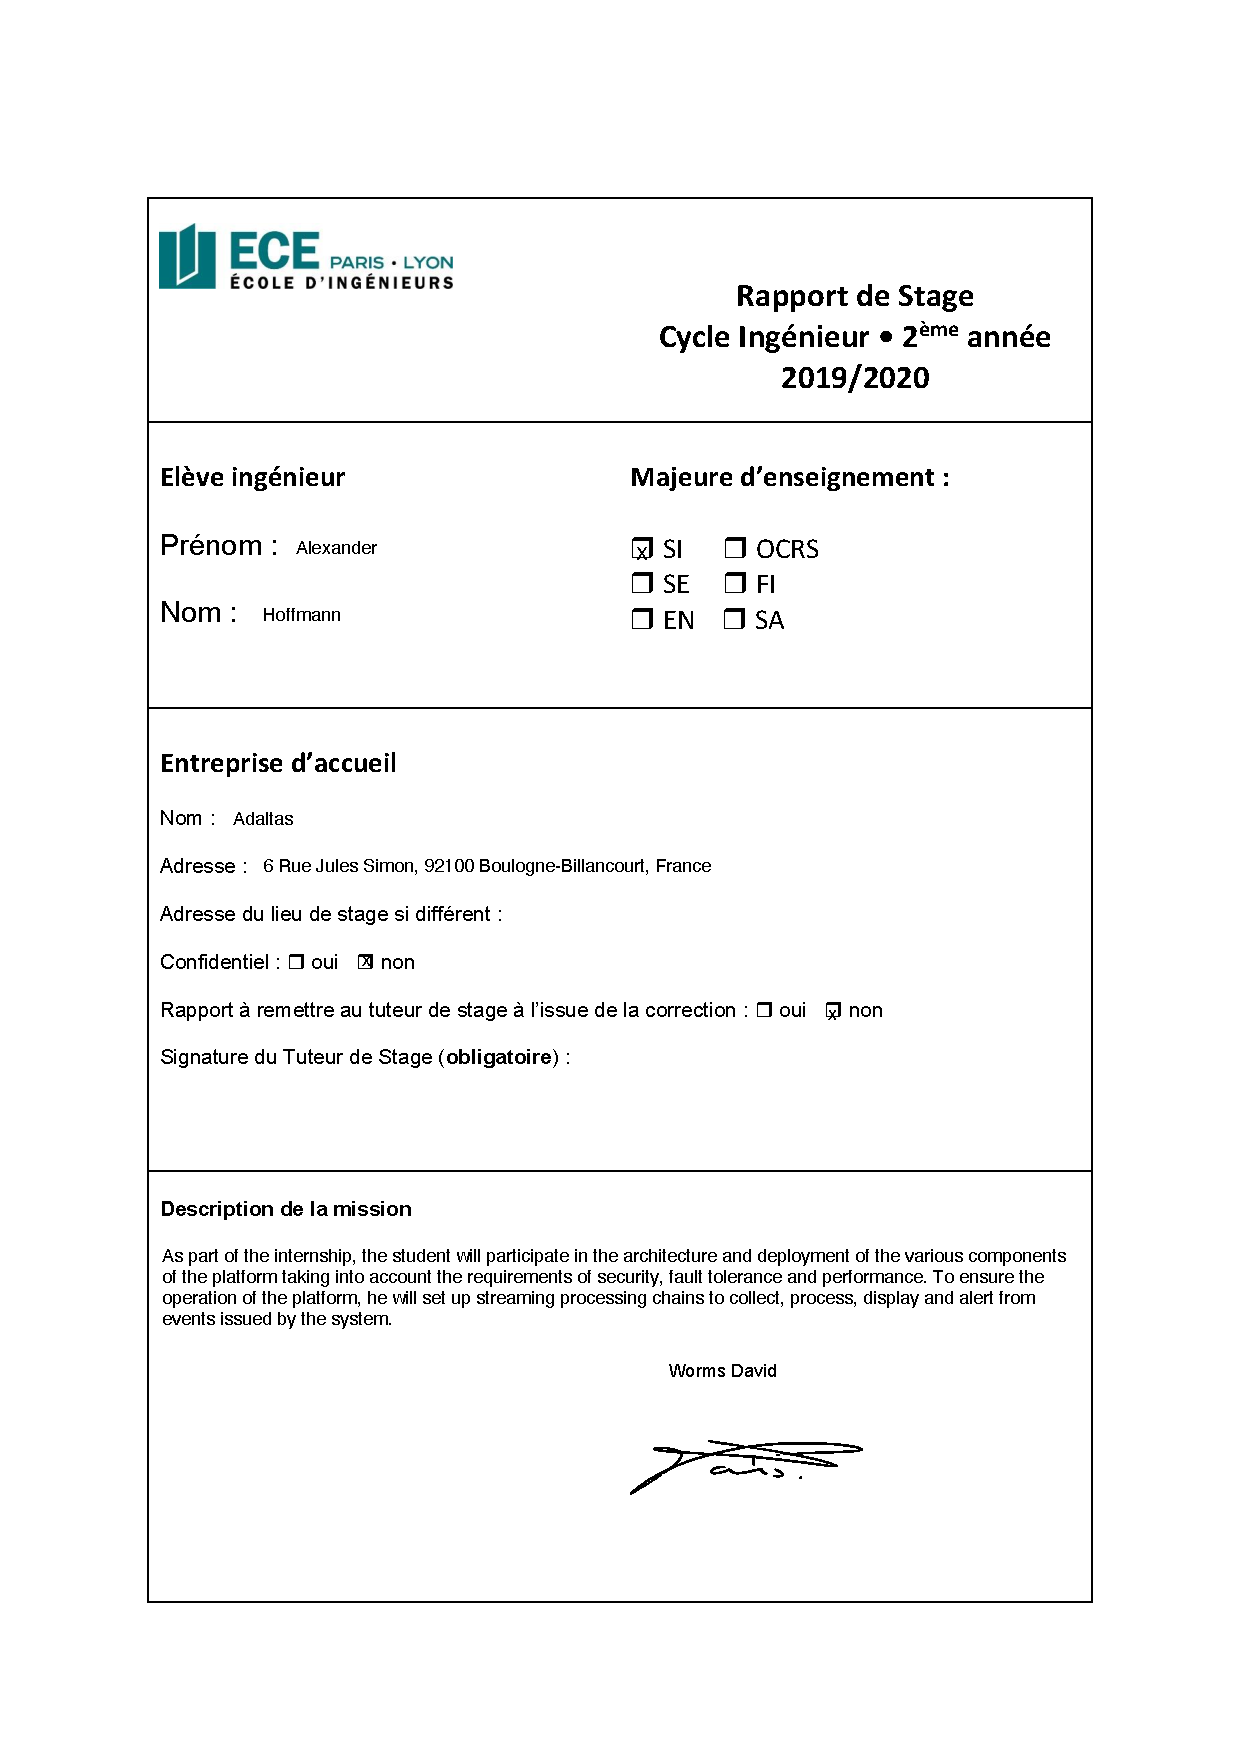
\includepdf[pages=-]{assets/pdf/title.pdf}

\maketitle

\chapter*{Remerciements}

Les premiers pas dans le monde du travail se font rarement seul et sans aide ni soutien. Je souhaite remercier toutes les personnes ayant contribué à cette expérience professionnelle.\\

Je tiens tout d’abord à remercier toute l'équipe d'Adaltas pour son accueil, sa bienveillance et sa bonne humeur permanente. J'apprécie l'attention et la sollicitude qui m'ont été prodiguées par toute personne rencontrée.\\

Je voudrais ensuite exprimer ma sincère gratitude à David Worms, mon tuteur, pour la confiance qu’il a bien voulu m’accorder en acceptant de m'intégrer à Adaltas. Je le remercie pour sa grande disponibilité, sa patience, son soutien chaleureux et ses conseils avisés. Je tiens à lui exprimer ma profonde reconnaissance pour ses critiques constructives d’une rigueur absolue.\\

Mes remerciements s’adressent également à Prisca Borges pour son accueil, sa sympathie et ses conseils, ainsi qu'à Léo Schoukroun pour son encadrement et sa compréhension qu'il m'a accordé tout au long du stage.\\

En cette période inédite de crise sanitaire, j'ai eu la chance de pouvoir travailler avec une entreprise qui a su s'adapter aux difficultés posées par les mesures nécessaires à la protection de ses collaborateurs. Je suis reconnaissant d'avoir pu effectuer mon stage dans les meilleurs conditions possibles.

\chapter*{Résumé}

Ce document décrit mon stage de 2ème année du cycle ingénieur effectué au sein de l'entreprise Adaltas. Adaltas est une équipe de consultants experts en Open Source, Big Data et systèmes distribués. La société fournit à ses clients un savoir faire reconnu sur la manière d'utiliser les technologies pour convertir leurs cas d'usage en projets exploités en production, sur la façon de réduire les coûts et d'accélérer les livraisons de nouvelles fonctionnalités.\\

Au sein de cette structure, j'ai eu la chance d'évoluer en tant que développeur. J'ai travaillé sur Nikita\footnote{\href{https://github.com/adaltas/node-nikita}{https://github.com/adaltas/node-nikita}}, une librairie d’automatisation pour le déploiement de systèmes pour \gls{nodejs}. Ce logiciel a été conçu dans le but d'aider les développeurs et les opérateurs à déployer des infrastructures et des logiciels Big Data de manière flexible et idempotente.\\

L'objectif de ce stage était de contribuer au développement d'un projet Open Source et ainsi d'en apprendre plus sur cet axe de valorisation. Adaltas est une société “open”. Son engagement se construit sur les fondations d’un code source ouvert, d’une collaboration ouverte, de standards ouverts et d’une formation ouverte. Il s'agit d'une façon de penser et de travailler à laquelle j'adhère fortement. C'est également l'une des raisons pour lesquelles j'ai choisi d'effectuer mon stage chez Adaltas.\\

\noindent\textbf{Mots clés} : big data, déploiement, devops, infraops.

\begingroup
\hypersetup{linkcolor=black}
\listoffigures
\tableofcontents
\newpage
\endgroup

\chapter*{Introduction}
\addcontentsline{toc}{chapter}{Introduction}

Mon intérêt pour la data science et plus généralement pour l’informatique et les nouvelles technologies m’ont amené à chercher un stage dans une société qui en a fait son coeur de métier. Le début de ma recherche de stage a été le mois de juillet 2019. J'ai envoyé des candidatures à plus d'une centaine d'entreprise dont Google, Amazon, Facebook et Apple. J'ai eu la chance de passer des entretiens techniques chez trois des entreprises citées précédemment. Sans trop entrer dans les détails, les épreuves comportent des questions algorithmiques appliquées à des problèmes ludiques qu'il s'agit de résoudre dans une durée impartie. Florent Diedler, un enseignant en informatique à l'ECE, m'a d'ailleurs beaucoup aidé lors de la préparation à ces entretiens. N'ayant eu aucune proposition de stage, j'ai continué mes recherches. C'est durant un cours de \gls{devops} animé par Gregor Jouet, consultant chez Adaltas, que j'ai découvert cette entreprise, ses méthodologies et sa culture. Aux alentours du mois de novembre, alors que nous travaillions sur un projet \gls{devops}, Gregor Jouet a invité les élèves intéressées par les technologies data science et big data à envoyer lui envoyer leur CV. Quelques semaines plus tard, j'ai reçu un appel de David Worms, dirigeant de la société Adaltas, qui m'a proposé un entretien. C'est dans ce contexte qu'est parvenue ma demande de stage à Adaltas qui a décidé d'accepter ma candidature.\\

Ce document présente les travaux et missions effectués au sein de l'entreprise Adaltas durant mon stage se déroulant du 14 avril au 30 août 2020, ceci représentant une durée totale de 4 mois et demi. Dans le cadre du stage, j'ai pu participer à l’architecture et au déploiement des différents composants d'un cluster en prenant en compte les impératifs de sécurité, de tolérance aux pannes et de performances. Pour assurer l’exploitation de la plateforme, j'ai mis en place des chaînes de traitement en streaming pour collecter, traiter, afficher et alerter à partir des évènements émis par le système.\\

La thématique de ce stage s’inscrit dans un contexte d’appréhension et d'approfondissement du monde de l’entreprise. Dans ce rapport, nous présenterons dans un premier temps le contexte du stage, c’est-à-dire que nous décrirons l’entreprise d’accueil, nous étudierons son secteur d’activité et sa culture. Dans un second temps, nous expliquerons les différents aspects de ma mission et les attentes de l'entreprise. Finalement, nous verrons les compétences et qualités acquises sur cette mission ainsi que ma valeur ajoutée pour l'entreprise.

\chapter{Présentation de la structure d'accueil: Adaltas}

Fondée en 2004, Adaltas est une société d’expertise en High Tech construite à partir de deux idées :
\begin{itemize}
  \item[--] l’innovation comme facteur de différenciation décisif pour les entreprises;
  \item[--] la capacité à mobiliser les meilleurs talents comme condition de succès.\\
\end{itemize}

\begin{figure}[H]

\includegraphics[scale=0.4]{assets/img/logo-adaltas.png}
\centering
\caption{Logo d'Adaltas représentant un oiseau. Adaltas signifie "vers le haut".}
\label{fig:logo-adaltas}
\end{figure}

Adaltas aide ses clients à s’orienter dans le monde en perpétuelle évolution de l’Open Source, leur donnant les clés pour développer les meilleures solutions, qu’il s’agisse simplement d’écrire une application ou d’élaborer une plateforme de traitement stratégique à plus long terme. L'entreprise se définit comme un acteur du Big Data autour des technologies \gls{hadoop} et \gls{nosql}.

Les équipes apportent une expertise sur l’analyse et le traitement des données, leur gouvernance, le développement et la gestion opérationnelle. Les consultants adhèrent à la culture \gls{devops} et ils sont formés à la méthodologie \gls{sre}\footnote{\href{https://landing.google.com/sre/}{What is Site Reliability Engineering (SRE)?}}. Ils accompagnent leur client dans la mise en place d’infrastructures et d’applications résilientes, conscients des rapides innovations apportés par la communauté Open Source et de la nécessaire stabilité des systèmes.

L'expertise d'Adaltas dans le domaine Big Data a commencé dès 2009 par l'accompagnement de la société EDF et la collecte des données Linky dit compteurs intelligents. En 2012, la société a entrepris l’exploitation d'une plateforme commune à l'ensemble du groupe EDF avec la mise à disposition des composants de l’éco-système Hadoop. Le nombre de composants s'est élargi avec le temps ainsi que les services et les cas d’usage qui ont accosté sur la plateforme sécurisé et multi-tenante.

Depuis 2014, l’équipe s’est élargie en accueillant des talents majoritairement formés à l’ECE, école dans laquelle Adaltas est à l’initiative du programme Big Data. Adaltas donne également des cours au Data Science Tech Institute\footnote{\href{https://www.datasciencetech.institute/}{https://www.datasciencetech.institute/}} et à l’Université Paris-Sorbonne.

\section{Objectifs de l'entreprise}

L’acquisition d’un cluster à forte capacité répond à la volonté d’Adaltas de construire une offre de type \gls{paas} pour disposer et mettre à disposition des plateformes de Big Data et d’orchestration de conteneurs. Les plateformes sont utilisées pour l’acquisition de nouvelles compétences, l’évaluation de nouvelles technologies, l’utilisation d’outils \gls{devops} et la mise à disposition d’environnements de développement, de PoCs et d’exploitation. Elles hébergent des Data Lakes, des DataLabs, des traitements et des modèles de Data Science, des outils orientés \gls{devops} ou encore des services applicatifs. L’objectif est de porter cette offre à maturité.

Dans le cadre de ses cours et formations, Adaltas s'intéresse au domaine Big Data et Data Science. Les cours effectuées au seins des différents établissements ont pour objectif de trouver des jeunes talents pour les faire monter en competence. Ainsi, la société cherche à recruter et former ses futurs consultants le plus tôt possible afin qu'ils soient opérationnels dès la fin du stage de dernière année d'école.

\section{Une entreprise "open"}

Adaltas est une société “open”. Leur engagement se construit sur les fondations d’un code source ouvert, d’une collaboration ouverte, de standards ouverts et d’une formation ouverte.

Les entreprises et les gouvernements utilisent les technologies Open Source pour remplacer les solutions propriétaires. Initialement, ces acteurs ont été attirés par les réductions de coût et la promesse de s’affranchir de la dépendance d’un éditeur. L’Open Source est désormais central à la transformation digitale avec des avantages avérés dans la sécurité, la qualité, la personnalisation, la flexibilité, l’intéropérabilité, l’auditabilité et le soutien.

Adaltas maintient près de 50 dépôts Open Source sur \gls{github} et encourage chaque développeur et client à contribuer à ces projets.

\section{La culture d'Adaltas}

Adaltas préserve un esprit familial qui privilégie toujours une vision à long terme. L'entreprise a pour vocation d’assurer le développement de chacun de ses consultants dans le respect de leur identité et de leur autonomie en mettant à disposition toutes les ressources nécessaires. Chaque service ou fonctionnalité proposé est le fruit d’une collaboration où chacun contribue aux idées des autres. L'objectif principal est de créer les meilleures expériences possibles pour les clients.

Le respect de ces valeurs est l’une des clefs de la performance d'Adaltas, de son ancrage dans l’air du temps et dans la société qui l'entoure.

\section{Par rapport à l'épidémie de Covid-19}

La réponse d'Adaltas face à l'épidémie de Covid-19 qui a touché la France au début de l'année 2020 était remarquable. La mise en place du télé-travail durant la période de confinement n'a pas affecté le déroulement de mon stage. Au contraire, j'ai apprécié la flexibilité apportée par le télé-travail et j'ai observé une augmentation de ma productivité durant cette période. Suite au déconfinement, j'ai demandé à continuer à travailler à distance. Au vu de mes prestations, David Worms a accepté ma requête.

\chapter{Présentation de la mission}

La mission principale de mon stage se concentrait autour du développement du logiciel d'automatisation de déploiement Nikita. Plus précisément, il s'agissait de migrer plusieurs packages, modules et actions ainsi que de refactor une partie du code vers une nouvelle version du logiciel.

\section{Cahier des charges}

Sur la base des différents objectifs présentés précédemment, un cahier des charges a été établi mi-avril 2020 par David Worms. Les activités précisées sont les suivantes : 

\begin{enumerate}
  \item Refactoring du code source du package \texttt{engine} afin d'en améliorer la lisibilité et, par voie de conséquence, la maintenance, et à le rendre plus générique.
  \item Migration des actions du module \texttt{file}, initialement contenue dans le package \texttt{core}, vers son propre package.
  \item Amélioration de la documentation dans les packages \texttt{engine} et \texttt{file} dans le but de la rendre plus complète et compréhensible.
  \item Conception de tests unitaires permettant de vérifier le bon fonctionnement des packages \texttt{engine} et \texttt{file}.
  \item Délivrance d'un rapport de stage à l'ECE Paris et à Adaltas.
\end{enumerate}

\section{Planning}

Le découpage temporel des missions proposé au début du stage est décrit sur la figure \ref{fig:planning}. Ce planning a été formulé en fonction de ma progression prévisionnelle de l'apprentissage des technologies nécessaires au développement de Nikita. Lesdites technologies seront étudiées en détails ci-après.

\begin{figure}[h]
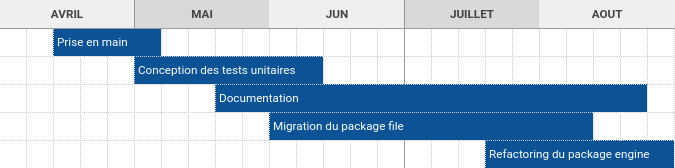
\includegraphics[scale=0.6]{assets/img/planning.png}
\centering
\caption{Planning sous forme de diagramme de Gantt}
\label{fig:planning}
\end{figure}

\chapter{Déroulement de la mission}

Cette partie décrit les activités réalisées dans le cadre du stage. La plupart d'entre elles ont été réalisées en parallèle. La description "chronologique" qui suit est donc très relative.

\section{Présentation de Nikita}

Nikita est une librairie d’automatisation pour le déploiement de systèmes pour \gls{nodejs}. Le logiciel est développé en \gls{javascript}. Le développement a commencé lorsqu'Adaltas a déployé un cluster \gls{hadoop} pour l’un de ses clients en 2011. Les actions Nikita sont variées : créer un dossier, générer un fichier, initier un service systemd, ajouter une règle de pare-feu iptable, etc.

Nikita est organisé comme un seul et unique dépôt multi-packages (monorepo) hébergé sur \gls{github}\footnote{\href{https://github.com/adaltas/node-nikita}{https://github.com/adaltas/node-nikita}}. Il comprend le moteur de base, les actions des utilisateurs et les fonctions utilitaires. Tous ces éléments sont associés à leurs tests unitaires. Lerna\footnote{\href{https://github.com/lerna/lerna}{https://github.com/lerna/lerna}} est utilisé pour diviser le projet en packages indépendants. Cela permet d'optimiser les besoins en temps et en espace, permettant un refactoring massif, une mise à jour et un enrichissement des fonctionnalités plus efficace. La figure \ref{code:example} représente un exemple d'une action Nikita.

\begin{figure}[H]
\begin{lstlisting}[language=JavaScript]
nikita = require('nikita')
nikita.call({
  who: 'leon'
}, function({options}){
    console.info(options.who)
  }
)
\end{lstlisting}
\centering
\caption{Exemple de code Nikita}
\label{code:example}
\end{figure}

\subsection{Les packages}

Comme évoqué précédemment, Nikita est divisé en plusieurs packages. Chaque package a un domaine d'application spécifique. Par exemple, le package \texttt{core} comporte les actions génériques, il permet de travailler sur des objets \gls{javascript}, modifier des fichiers, etc. Le package \texttt{docker} contient des actions liées à \gls{docker}. Le package \texttt{file}, que je suis chargé de migrer, comporte des actions permettant de travailler sur le système de fichier. Par exemple, nous pouvons y trouver des fonctions pour créer un fichier, supprimer un répertoire, télécharger un document, etc.

\subsection{Les actions}

Une action est un élément fondamental dans Nikita. Il s'agit essentiellement d'une fontion que nous appelons \texttt{handler} et des metadonnées associées appelées \texttt{options} ou \texttt{config}. Les actions génériques et bas niveau se situent dans le package \texttt{engine}. Par exemple, dans \texttt{engine/src/actions/fs/base/mkdir.coffee.md}, nous trouvons l'action \texttt{mkdir} qui permet de créer un répertoire.

\section{Prise en main de Nikikta}

Ma première activité consistait à comprendre la logique de Nikita. Pour pouvoir m'approprier et faire évoluer ce logiciel, il me fallait tout d'abord comprendre sa manière de fonctionner. Pour ce faire, j'ai dans un premier temps suivi les instructions du tutoriel\footnote{\href{https://nikita.js.org/about/tutorial/}{https://nikita.js.org/about/tutorial/}} disponible sur le site internet. L'utilisation de Nikita nécessite l'installation de \gls{nodejs} et de \gls{npm} ou \gls{yarn}. Ayant déjà utilisé ces technologies dans plusieurs cours dispensés à l'ECE, j'étais familié avec l'environnement de développement de Nikita fort de quoi j'ai pu avancer à un rythme plus soutenu durant ce tutoriel. Le fonctionnement de Nikita est fondé autour des fichiers. Toutes les actions de la librairie touchent de près ou de loin à un fichier. Ainsi, il est possible de suivre le déroulement d'une session Nikita en observant les modifications effectuées sur les différents fichiers.

Nikita est executé par le moteur \gls{nodejs}. Cela signifie que le développement du logiciel nécessite des connaissances en \gls{javascript}. Fort heureusement, les enseignements de l'ECE couvrent également les bases de ce langage de programmation. De surcroît, j'ai utilisé à titre personnel le langage \gls{javascript} pour plusieurs projets. J'avais donc des fondations solides pour me lancer dans le code source. C'est en tout cas ce que je pensais. Il s'avère que, même s'il est possible d'utiliser Nikita en travaillant en \gls{javascript}, le code source est écrit en \gls{coffeescript}, un langage de programmation, qui se compile en \gls{javascript}. En d'autres termes, le code écrit en \gls{coffeescript} est transformé en \gls{javascript}. Cela étant dit, les syntaxes entres ces deux langages sont très similaires comme le montre la figure \ref{code:jscoffeecomparison}.

\begin{figure}[H]
\begin{minipage}{0.45\textwidth}
\begin{lstlisting}[language=JavaScript]
a = 2
square = (x) -> x * x
b = square a
console.log b // 4
\end{lstlisting}
\end{minipage}\hfill
\begin{minipage}{0.45\textwidth}
\begin{lstlisting}[language=JavaScript]
var a, b, square;
a = 2;
square = function(x) {
  return x * x;
};
b = square(a);
console.log(b); // 4
\end{lstlisting}
\end{minipage}\hfill
\centering
\caption{Comparaison de code \gls{javascript} et \gls{coffeescript}}
\label{code:jscoffeecomparison}
\end{figure}

\gls{coffeescript} a une syntaxe très claire et se prête parfaitement à l'aspect déclaratif de Nikita. Somme toute, le code source ressemble à du \gls{yaml}, ce qui le rend beaucoup plus lisible tout en préservant les avantages d'un langage procédural tel que le \gls{javascript}. Un autre avantage de \gls{coffeescript} est qu'il permet d'intégrer la documentation liée à une action directement dans le code source.

Ma première mission pour prendre en main Nikita était la migration d'une action de Nikita Arch\footnote{\href{https://github.com/adaltas/node-nikita-arch}{https://github.com/adaltas/node-nikita-arch}}, un logiciel de déploiement pour le système d'exploitation \gls{arch}, vers Nikita dans le package \texttt{core}. Les actions contenues dans le dépôt Nikita Arch sont indépendantes et, de façon générale, plus simple que celles sur Nikita. J'ai ainsi pu me familiariser avec la logique et syntaxe du logiciel. Dans ce cas précis, je n'ai pas eu à écrire de nouveau code. Je devais prendre le code existant, le copier vers le package \texttt{core} et modifier certaines lignes relatives à l'environnement d'exécution. J'étais également chargé d'écrire des tests unitaires. Il s'agit d'une procédure permettant de vérifier le bon fonctionnement d'une partie précise du logiciel (appelée « unité » ou « module »). Reprenons l'exemple de la figure \ref{code:jscoffeecomparison}. Ce code décrit une fonction \texttt{square} dont le but est d'élever au carré l'entier qui est passé par paramètre. Le test unitaire le plus basique serait de vérifier que si l'on envoie le chiffre 3 dans cette fonction, cette dernière retourne le chiffre 9. L'objectif final est de "blinder" le code, c'est-à-dire vérifier qu'il se comporte comme le développeur l'a prévu. L'éciture de tests unitaires permet de trouver rapidement les erreurs au sein du code, de sécuriser la maintenance et finalement de documenter le code. Ils peuvent servir de complément à l'\gls{api}, il est très utile de lire les tests pour comprendre comment s'utilise une méthode. De plus, il est possible que la documentation ne soit plus à jour, mais les tests eux correspondent à la réalité de l'application. C'est d'ailleurs ce que m'avait conseillé mon maître de stage durant ma montée en compétences sur le logiciel Nikita.

\chapter*{Conclusion}
\addcontentsline{toc}{chapter}{Conclusion}

Fort des éléments énoncés précédemment, ce stage technique effectué au sein de l’entreprise Adaltas constitue une expérience des plus enrichissantes étant donné la complexité technique des missions auxquelles j'ai pu prétendre. Outre l’aventure humaine que j’eus la chance et le privilège de vivre, ce stage m’apprit le sens de la rigueur, du professionnalisme, ainsi que l’importance du temps et de son agencement. Grâce à cette expérience, j’ai acquis des compétences telles que le fonctionnement de (.................). De plus, les différentes missions effectuées m’ont permis d’accroître ma volonté de savoir et de connaissance, notamment dans le domaine du Big Data.

\clearpage

\printglossaries

\end{document}

